\documentclass{article}
\usepackage[margin=1in]{geometry}
\usepackage{enumitem}
\usepackage{setspace}
\usepackage{amsmath}
\usepackage{amssymb}
\usepackage{physics}
\usepackage{graphicx}

\title{Math 180 Homework 4}
\date{11/8/2020}
\author{Jiaping Zeng}

\begin{document}
\setstretch{1.35}
\maketitle

\begin{itemize}
      \item [6.4.1] Prove that $\chi(G)\leq 1+\max\{\deg_G(x):x\in V\}$ holds for every (finite) graph $G=(V,E)$.\\
            \textbf{Answer}: By induction on the number of vertices $n=\abs{V}$.\\
            Base case: $n=1$; since there is only a vertex, $\chi(G)=1$. In addition, we have $\max\{\deg_G(x):x\in V\}=0$ as there is no edge in a graph with a single vertex. Therefore $\chi(G)=1\leq 1+0$ is indeed true.\\
            Inductive step: Suppose the statement holds for every finite graph with $n$ vertices, we will show that it also holds for every graph with $n+1$ vertices. Let $G$ be a graph with $n+1$ vertices. We can remove an arbitrary vertex $v$ and its edges, giving us $G-v$, which has $n$ vertices. Let $m_G=\max\{\deg_G(x):x\in V\}$ and $m_{G-v}=\max\{\deg_{G-v}:x\in V\}$; by inductive hypothesis, we have $\chi(G-v)\leq 1+m_{G-v}$. Since $\deg_G(v)\leq m_G$, we can examine the following two scenarios:
            \begin{itemize}
                  \item [1.] $m_G=m_{G-v}$, which implies that the vertex with the highest degree in $G-v$ is not connected to $v$ in $G$, or else we would have $m_G=m_{G-v}+1$. Then we can assign $v$ the color of that vertex, giving us $\chi(G)\leq 1+m_{G-v}=1+m_G$.
                  \item [2.] $m_G\geq m_{G-v}+1$, then we can assign $v$ a new color, giving us $\chi(G)\leq 2+m_{G-v}\implies\chi(G)\leq 1+m_G$.
            \end{itemize}
            Therefore $\chi(G)\leq 1+\max\{\deg_G(x):x\in V\}$ holds by mathematical induction.
      \item [7.1.2]
            \textbf{Answer}: Suppose that when the tourist was descending along the trail, there was another tourist ascending along the same trail in the same fashion that the first tourist did on the day before. Then since the paths of both tourists are continuous, they must intersect at some point. The intersection point is the place that the tourist passed through at the same time on both days.
      \item [7.2.7] Let $n$ be a natural number that is not divisible by the square of any integer greater than 1. Determine the maximum possible size of a set of divisors of $n$ such that no divisor in this set divides another (i.e. $\max\abs{M}$, where $x\in M\Rightarrow x\mid n$ and $x,y\in M,x\neq y\Rightarrow x$ doesn't divide y).\\
            \textbf{Answer}: Let $D=\{d_1,\ldots,d_n\}$ be the set of all divisors of $n$ and $M=\{p_1,\ldots,p_m\}$ be the set of all prime factors of $n$. Then each $d_i\in D$ can be written as a product of a subset of $P$. Then by Sperner's Theorem, the maximum possible size of a set of divisors is $\binom{\abs{P}}{\lfloor\abs{P}/2\rfloor}$.
      \item [5.1.1] Draw all trees with vertex set $\{1,2,3,4\}$, and all pairwise nonisomorphic trees on 6 vertices.\\
            \textbf{Answer}: As shown below:
            \begin{center}
                  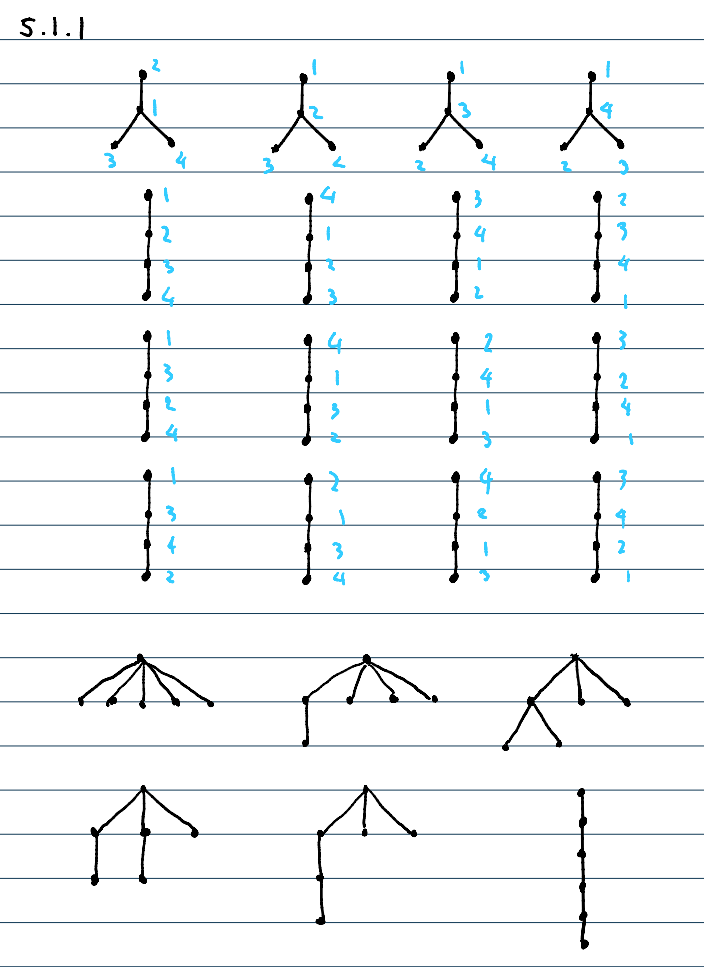
\includegraphics[width=4in]{5-1-1.png}
            \end{center}
      \item [5.1.2] Prove that any graph $G=(V,E)$ having no cycles and satisfying $\abs{V}=\abs{E}+1$ is a tree.\\
            \textbf{Answer}: By definition, a tree is a connected graph containing no cycle. Since we already have that $G$ contains no cycle, we need to show that $G$ must be connected. Suppose that $G$ is not connected, then there must exist at least 2 components. Let the components have $p$ and $q$ vertices respectively, we then have $p+q=\abs{V}$. Since $G$ does not have a cycle, the components can have at most $p-1$ and $q-1$ edges, so $G$ can have at most $p+q-2=\abs{V}-2$ edges, i.e. $\abs{E}=\abs{V}-2$. However, we have $\abs{V}=\abs{E}+1\implies\abs{E}=\abs{V}-1$. Therefore $G$ must be connected by contradiction and $G$ is therefore also a tree.
      \item [5.1.4] Prove that a graph on $n$ vertices with $c$ components has at least $n-c$ edges.\\
            \textbf{Answer}: By induction on $c$.\\
            Base case: $c=1$; then the graph is connected. Such graph with as few edges as possible is a path, with has exactly $n-1$ edges.\\
            Inductive step: Suppose that all graphs on $n$ vertices with $c$ components have at least $n-c$ edges, we want to show that all graphs on $n$ vertices with $c+1$ components have at least $n-c-1$ edges. By inductive hypothesis, since $n-c$ edges is the minimum number of edges a graph with $c$ components can have, we can simply disconnect any edge in the graph to create an extra component. Then we have a graph with $c+1$ components and $n-c-1$ edges. In addition, we cannot remove any additional edge as that would create extra components, so $n-c-1$ is minimum number of edges a graph with $c+1$ components can have.\\
            Therefore a graph on $n$ vertices with $c$ components has at least $n-c$ edges.
      \item [P9]
            \begin{itemize}
                  \item [(a)]
                        \textbf{Answer}: A crown graph has chromatic number 2 since it is bipartite. For a crown graph on 6 vertices, we can use the ordering $v_1,u_1,v_2,u_2,v_3,u_3$ and examine how the greedy algorithm behaves. The first vertex $v_1$ uses color 1, then $u_1$ will also use color 1 as it is not connected to $v_1$. Then $v_2$ uses color 2 since it is connected to $u_1$, which already has color 1. Similarly, $u_2$ also has to use color 2. Then $v_3$ needs to use color 3 since it is connected to both $u_1$ and $u_2$, which had already used the first 2 colors. Therefore the greedy algorithm gives us 3 colors in this case which is not optimal.
                  \item [(b)]
                        \textbf{Answer}: We can simply pick vertices from the two sets $\{v_1,v_2,\ldots,v_k\}$ and $\{u_1,u_2,\ldots,u_k\}$ in order and alternatingly, i.e. $v_1,u_1,v_2,u_2,\ldots,v_k,u_k$. This ordering will always provide a $k$-coloring as $v_i$ cannot use colors $1,\ldots,i-1$, since it is connected to $\{u_1,\ldots,u_{i-1}\}$ which used the first $i-1$ colors. Similarly, $u_i$ also cannot use colors $1,\ldots,i-1$. Therefore $v_k$ and $u_k$ must use the $k$th color, giving us a $k$-coloring.
            \end{itemize}
\end{itemize}
\end{document}